\begin{abstract}
Este trabajo consiste en el levantamiento y análisis del trazado de una red de media/baja tensión ubicada en Cabecera del Llano: 46181 Cra. 35A. Se desarrolló el levantamiento de un trazado de red desde la dirección mencionada como punto de inicio, por la carrera 35A en dirección norte-sur hasta 48178 Cra. 35A, y también desde el punto de inicio mencionado por la calle 48 en sentido oeste-este hasta 35a37 Cl. 48. Esto se realizó mediante inspección visual en campo. El objetivo de este levantamiento es analizar la distribución desde el transformador, identificar sus componentes visibles y seguir el recorrido de los conductores hasta la acometida del usuario final.
\end{abstract}

\section{Introducción}

\subsection{Justificación}
Aporta como construcción de conocimiento al identificar cómo está compuesto el sistema de distribución que llega al usuario final. Además, aporta información a la planificación urbana, ya sea identificando buenas prácticas o incumplimiento de normativas.

\subsection{Alcance y Delimitación}
Se especifica claramente que el estudio se limita a los circuitos de baja tensión derivados del transformador seleccionado en el punto de inicio en el barrio Cabecera del Llano, como se muestra en la ruta de la \textbf{Figura}~\ref{fig:ruta_estudio}. El análisis no incluye mediciones de carga o eléctricas, y tampoco se consideran equivalentes de la topología circuital.

\begin{figure}[H]
    \centering
    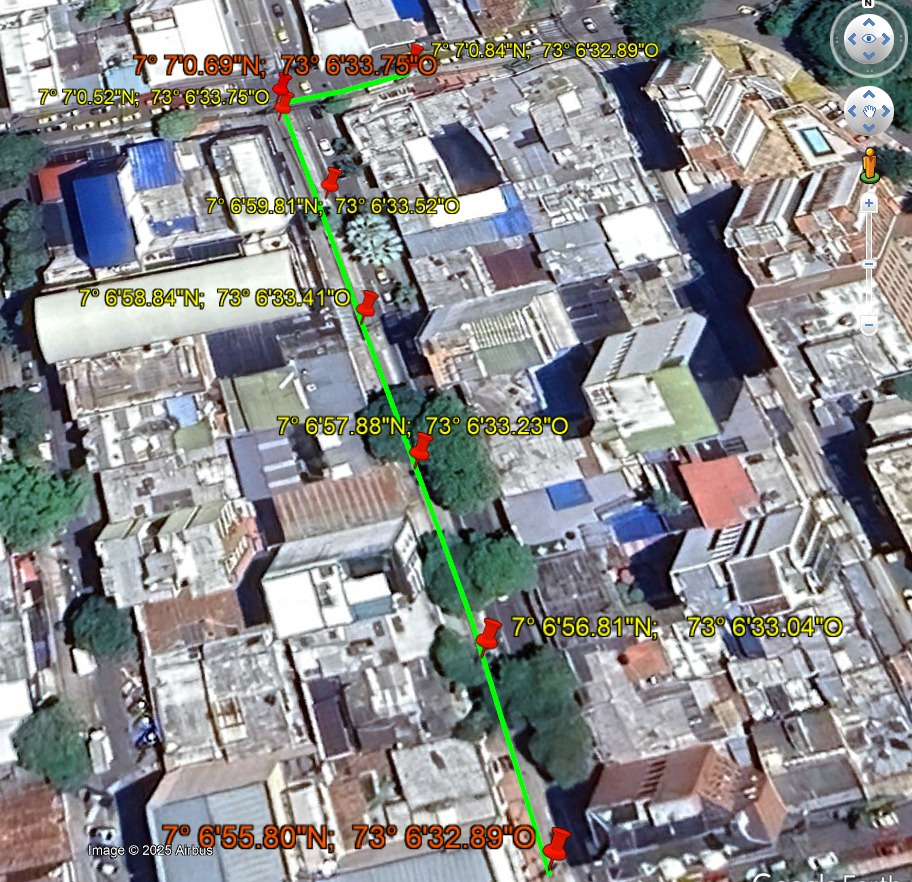
\includegraphics[width=0.43\textwidth, height=0.43\textwidth]{fig_/ruta}
    \caption{Vista satelital de la ruta de estudio en el barrio Cabecera del Llano. La línea verde traza el recorrido de la red de distribución eléctrica analizada, con marcadores rojos que indican las coordenadas geográficas de puntos clave inspeccionados en campo.}
    \label{fig:ruta_estudio}
\end{figure}


\section{Marco Teórico y Normativo}

En Colombia existen dos tipos de conexión para repartir la energía por todo el territorio: la principal es el SIN (Sistema de Interconectado Nacional). Bajo la Ley 143 de 1994, se menciona que en el SIN se establecen equipos de generación, red de interconexión, redes regionales e interregionales, redes de distribución y las cargas de los usuarios \cite{ley143_1994}. En este caso, nos interesa la última fase antes de que la carga llegue a los usuarios, la cual es la red de distribución, que en la misma ley se define como el conjunto de líneas y subestaciones con sus equipos asociados, destinado al servicio de los usuarios de un municipio o municipios adyacentes \cite{ley143_1994}.

Las tensiones que maneja el sistema de distribución local hacen parte de baja y media tensión, siendo la máxima tensión los 220 kV. Esto lo diferencia del STR (Sistema de Transmisión Regional), el cual opera bajo la misma tensión, sin embargo, este último no conecta con la carga final. Teniendo presente que en el Sistema de Distribución Local (SDL) se presentan las cargas inferiores a 220 kV correspondientes al nivel IV según la CREG \cite{creg}.

Es preciso aclarar las diferencias entre baja y media tensión. Se pueden diferenciar por su nivel, ya que para el nivel I es de baja tensión, y para los niveles II y III, son para media tensión \cite{creg}. Sin embargo, aunque se puede manejar el nivel IV, no es tan común en el SDL. Otra diferencia es el propósito de estos, ya que la media tensión se enfoca en la transmisión desde una subestación hasta el transformador que conecta las cargas de los usuarios, donde ya es de baja tensión, por lo cual está más enfocada al consumo de los usuarios. Por último, también se pueden diferenciar por el riesgo eléctrico que ambos proveen: en baja es mucho menor que en media, sin embargo, nunca es despreciable.

Otra parte importante es el tipo de conexión que pueda tener, que puede ser radial, en anillo o en malla. Para ello es importante tener en cuenta los puntos de conexión. Si se tiene solo una fuente, que es la subestación, la conexión radial es la indicada, ya que permite que la corriente fluya en una sola dirección. Si hay más de dos puntos de conexión, se puede hacer un circuito cerrado, con el cual se concreta la conexión en anillo. La última conexión es la de malla, esta es la más compleja, debido a que de un solo punto salen múltiples ramificaciones interconectadas que posteriormente culminan en distintos usuarios.

Según lo estipulado por el RETIE sobre la distribución, se deben tener transformadores con capacidades superiores a 3 kVA y se incluyen circuitos primarios y secundarios \cite{retie_2013}. Los primarios son los que provienen de las subestaciones o alimentadores, con capacidad de 7,6 kV a 44 kV. Por otro lado, los secundarios son aquellos que llegan a los usuarios, siendo de baja tensión, desde los transformadores de distribución hasta las acometidas de los usuarios \cite{retie_2013}. Adicionalmente, se establece un circuito especial para el alumbrado público, que debe estar conectado a transformadores no mayores a 75 kVA \cite{retie_2013}.

Con respecto a los postes, se estipula que la tensión de rotura que deben manejar debe ser superior a la suma de todas las cargas de rotura de las distintas líneas, previendo una modificación futura. Sin embargo, la modificación debe estar bien justificada, sin que esta (una nueva línea) supere la rotura establecida, la cual está principalmente en el rango de 250 a 510 kgf o superiores \cite{retie_2013}. Por otra parte, los postes deben ser de entre 6 a 7 metros de altura, especificando que los de 6 metros deben tener una rotura superior a 250 kgf \cite{retie_2013}. Para la seguridad, los postes metálicos o de concreto deben tener una conexión a tierra, con excepción de los destinados a baja tensión. Para culminar, la instalación debe tener una profundidad de 60 centímetros más el 10\% de la altura del poste \cite{retie_2013}.

Los conductores deben cumplir ciertos criterios para garantizar la seguridad de los usuarios. Se deja claro que los conductores aéreos pueden ser desnudos, pero deben ser semiaislados o aislados, y no se deben someter a más del 25\% de su tensión de rotura \cite{retie_2013}. Los conductores cubiertos, en rangos superiores a 46 kV, deben estar aislados en forma de PIN o de suspensión y deben tener protecciones DPS cuando se cambia a redes con conductores desnudos \cite{retie_2013}. Para los conductores subterráneos se deben usar ductos no higroscópicos (que no retienen ni atraen humedad). Estos ductos deben tener una distancia mínima de 0.20 metros a los ductos de agua o gas, y la profundidad debe ser la que indica la tabla 300.5 de la NTC 2050 \cite{ntc2050_1998}.

Finalmente, las distancias mínimas de seguridad de los postes y cableados están establecidas por el título 10, capítulo 5 del libro 3 del RETIE \cite{retie_2013}. Se menciona que la distancia de la parte más baja de un conductor hasta el techo de una casa no debe ser menor a 0,48 metros para tensiones inferiores a 1 kV. Sin embargo, esta distancia se puede ampliar hasta los 3,8 metros si la tensión llega hasta los 7,6 kV \cite{retie_2013}. La distancia próxima a los edificios, en zonas como terrazas, debe ser entre 1,7 y 2,3 metros para tensiones de máximo 7,6 kV \cite{retie_2013}. Se deja claro que la distancia vertical desde balcones o zonas de fácil acceso, a alturas de 2,45 metros, debe estar entre 3,5 y 4,1 metros, siempre y cuando la tensión sea inferior a 7,6 kV \cite{retie_2013}. Por último, en zonas peatonales, callejones y carreteras, la altura debe ser de más de 5 metros si la tensión es inferior a 1 kV, hasta 5,6 metros para tensiones no superiores de 7,6 kV \cite{retie_2013}.


\section{Resultados y Hallazgos}

A lo largo de la inspección de campo, se identificaron y documentaron varios componentes clave de la red de distribución eléctrica. 

La \textbf{Figura}~\ref{fig:doble_poste} muestra la estructura principal de la zona, compuesta por un doble poste que soporta un transformador de 125 [kVA] y la línea de media tensión. Se observan elementos como conectores bimetálicos, un aislador tensor cerámico para la red trenzada y crucetas de acero galvanizado.

Para el registro del consumo, se utilizan medidores eléctricos digitales como el que se ve en la \textbf{Figura}~\ref{fig:medidor}. Este equipo emplea tecnología electrónica para obtener un registro preciso de la energía activa. La infraestructura general se apoya en postes de concreto reforzado, esenciales para el transporte de energía desde las subestaciones, como se detalla en la \textbf{Figura}~\ref{fig:poste_concreto}.

Se encontraron distintas configuraciones de postes. La \textbf{Figura}~\ref{fig:poste_sencillo_cuadro} corresponde a un poste sencillo con una cruceta en forma de cuadro para la línea de media tensión, conectores aislados y un reflector LED para alumbrado público. Otra variación es la que se aprecia en la \textbf{Figura}~\ref{fig:poste_mt_bt}, donde un solo poste soporta tanto líneas de media como de baja tensión, además de cables de fibra óptica y TV. 

Finalmente, la \textbf{Figura}~\ref{fig:poste_acometida_edificio} ilustra un poste que, además de los elementos de distribución, incluye un medidor digital y un alimentador directo en media tensión para un edificio cercano. La densidad del cableado es evidente en la \textbf{Figura}~\ref{fig:poste_telecom}, donde un poste sostiene múltiples niveles de cables, principalmente de redes de baja tensión y telecomunicaciones.

\begin{figure}[H]
    \centering
    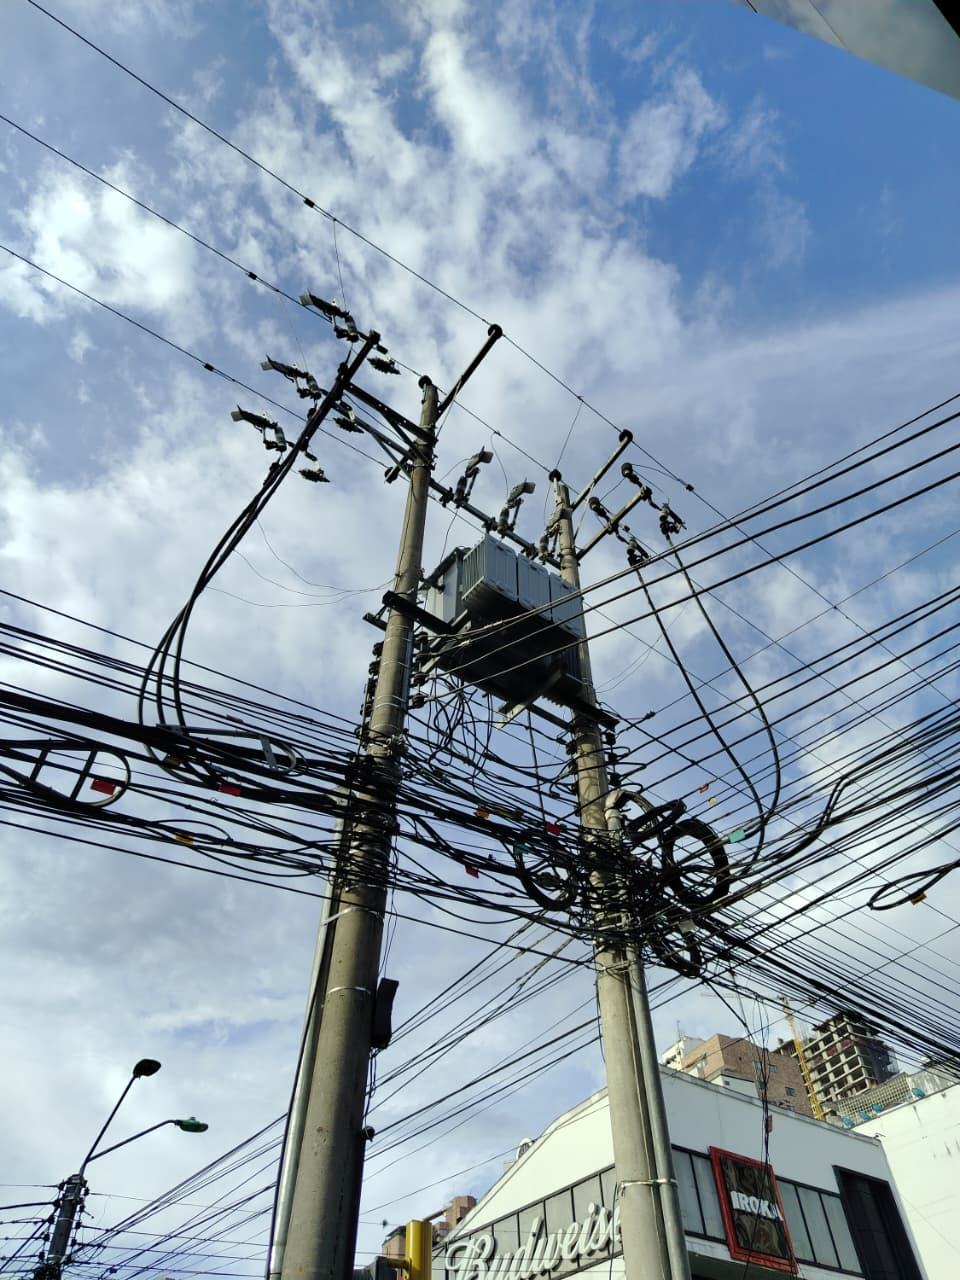
\includegraphics[width=0.43\textwidth, height=0.43\textwidth]{fig_/1.jpeg}
    \caption{Doble poste con transformador de 125 [kVA].}
    \label{fig:doble_poste}
\end{figure}

\begin{figure}[H]
    \centering
    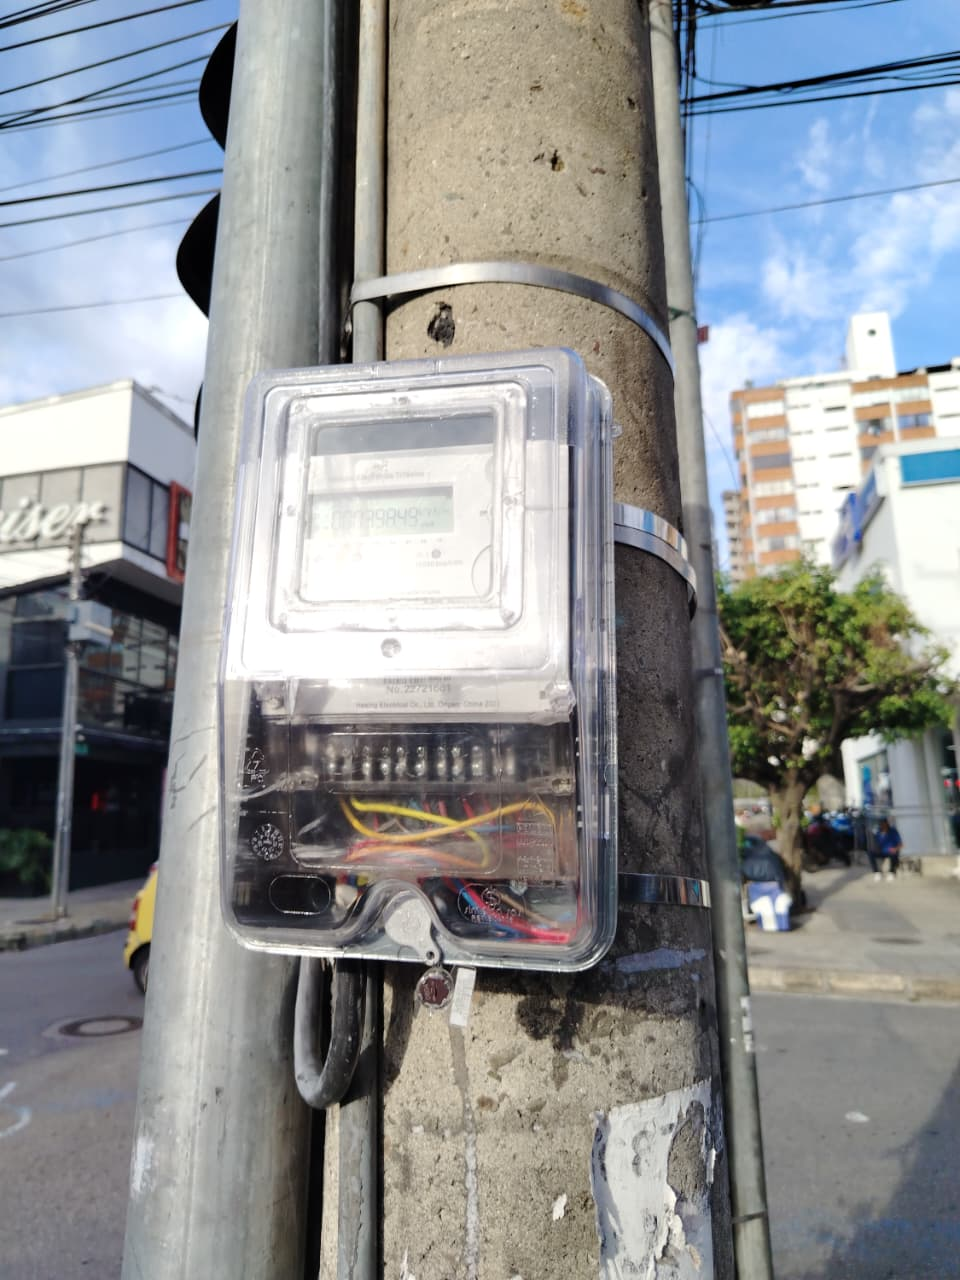
\includegraphics[width=0.43\textwidth, height=0.43\textwidth]{fig_/2}
    \caption{Medidor eléctrico digital.}
    \label{fig:medidor}
\end{figure}

\begin{figure}[H]
    \centering
    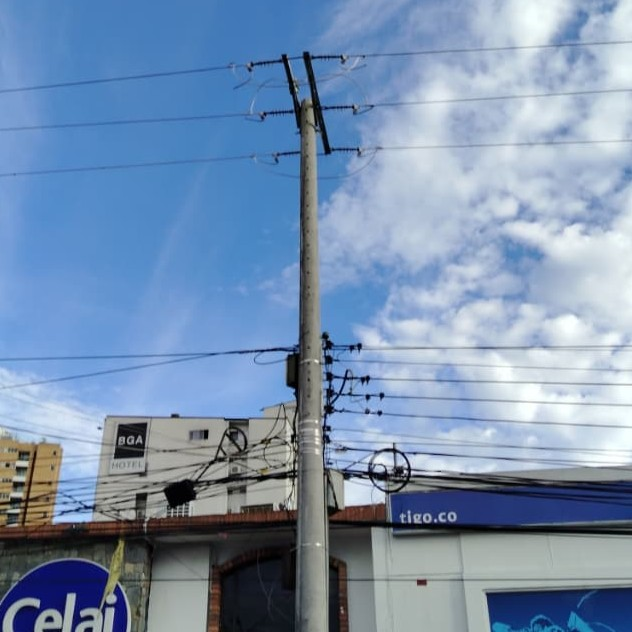
\includegraphics[width=0.43\textwidth, height=0.43\textwidth]{fig_/3}
    \caption{Poste de concreto reforzado.}
    \label{fig:poste_concreto}
\end{figure}

\begin{figure}[H]
    \centering
    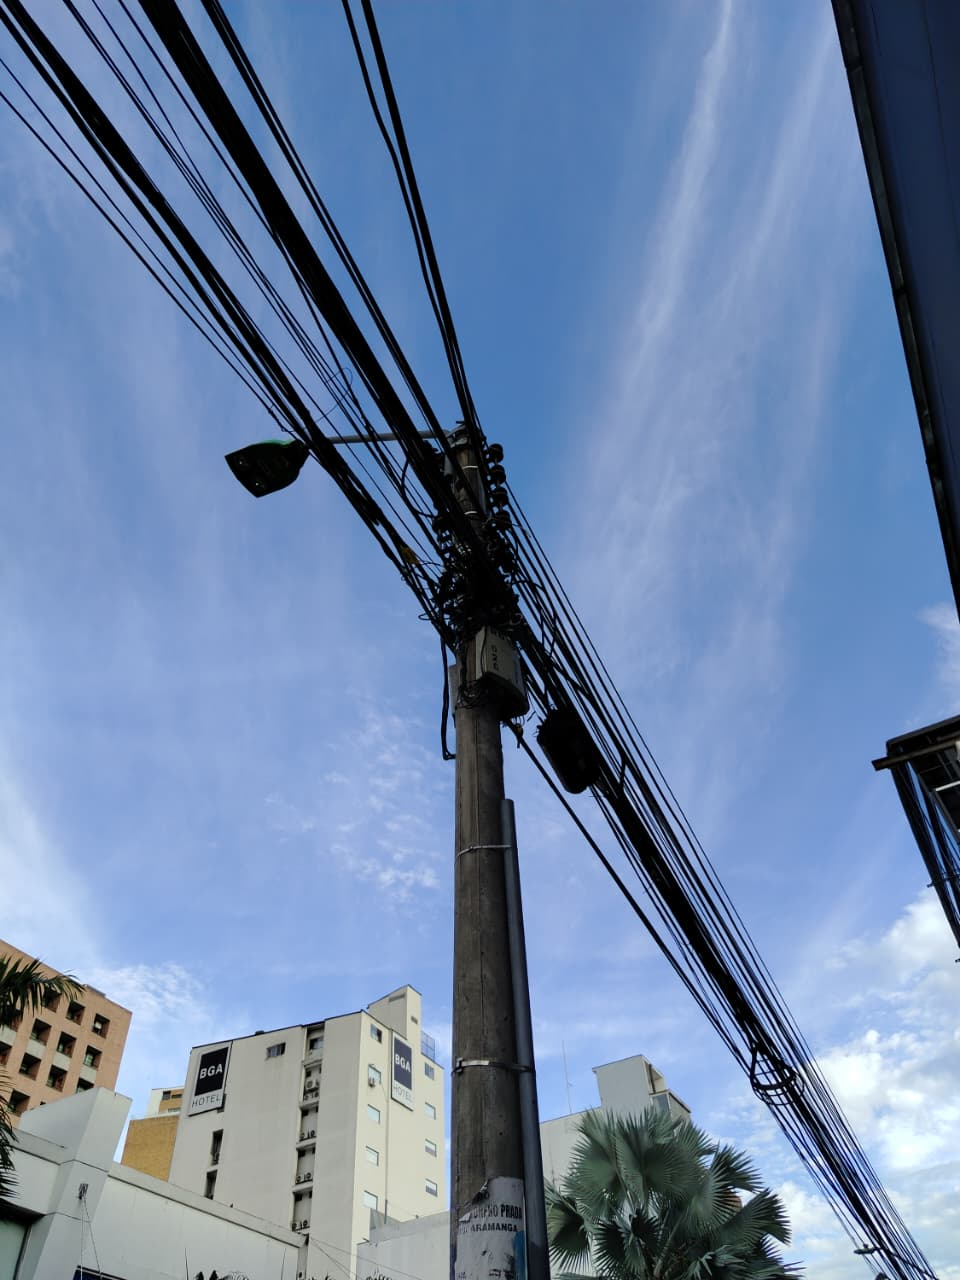
\includegraphics[width=0.43\textwidth, height=0.43\textwidth]{fig_/4}
    \caption{Poste sencillo con cruceta en cuadro.}
    \label{fig:poste_sencillo_cuadro}
\end{figure}

\begin{figure}[H]
    \centering
    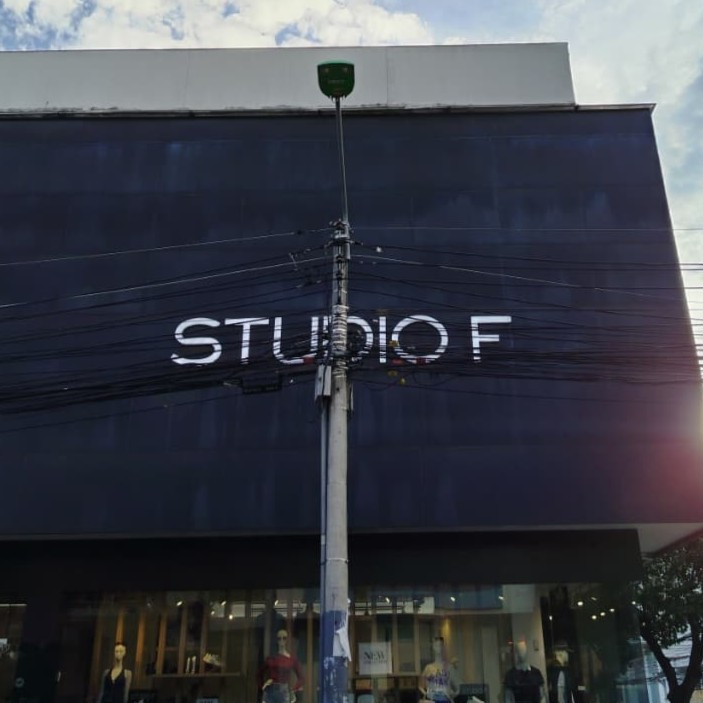
\includegraphics[width=0.43\textwidth, height=0.43\textwidth]{fig_/5}
    \caption{Poste con líneas de media y baja tensión.}
    \label{fig:poste_mt_bt}
\end{figure}

\begin{figure}[H]
    \centering
    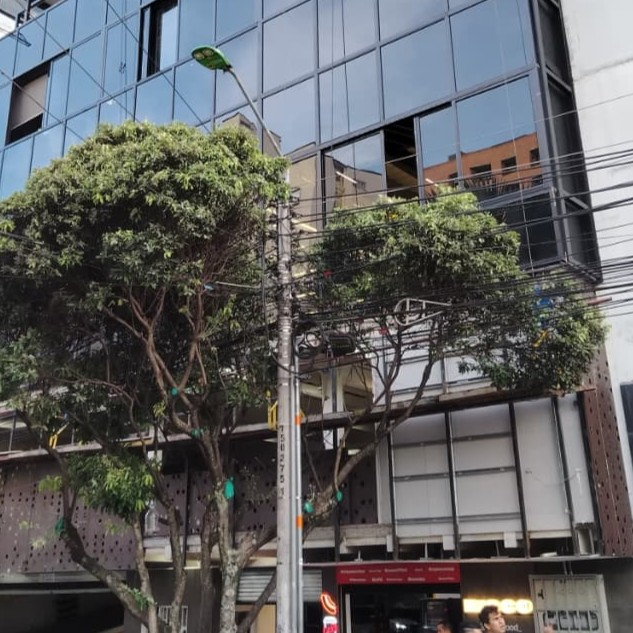
\includegraphics[width=0.43\textwidth, height=0.43\textwidth]{fig_/6}
    \caption{Poste con alimentador a edificio.}
    \label{fig:poste_acometida_edificio}
\end{figure}

\begin{figure}[H]
    \centering
    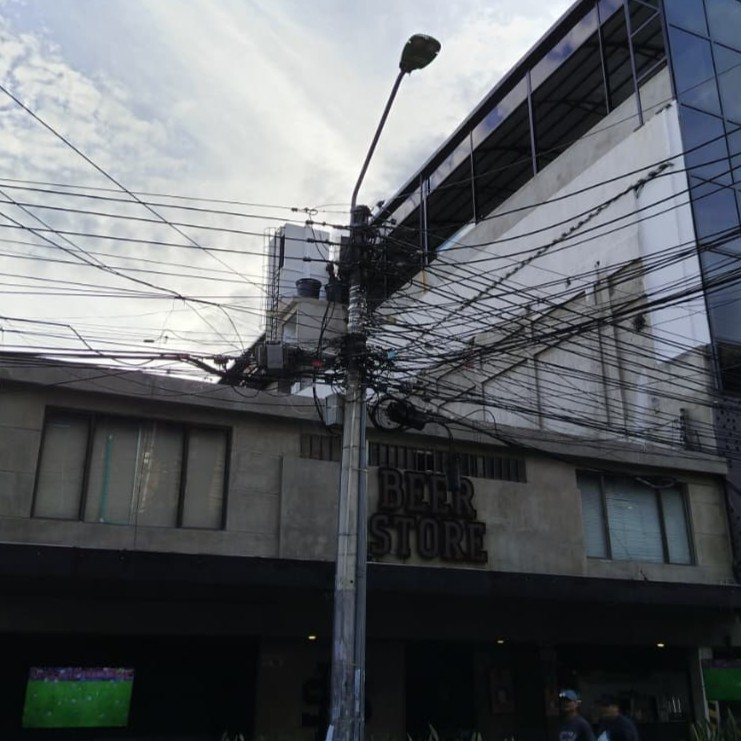
\includegraphics[width=0.43\textwidth, height=0.43\textwidth]{fig_/7}
    \caption{Poste con redes de BT y telecomunicaciones.}
    \label{fig:poste_telecom}
\end{figure} % Es buena idea mantener esto al final de la sección de figuras.

\section{Análisis y Discusión}

El transformador asignado para cubrir esa ruta es de 125 kVA. La zona en la que se encuentra es comercial y la demanda de energía es alta para su normal funcionamiento.

\subsection{Estado de la Infraestructura y Modernización}
Los elementos que hacen parte de la red de distribución en la ruta objeto de estudio poseen la incorporación de tecnología moderna, como medidores digitales y luminarias LED. En la parte de la medición, esto permite obtener datos de manera precisa y facilita la detección de fraude. En cuanto a las luminarias LED, ofrecen ahorro en el consumo de energía y poseen una vida útil que las hace viables para su implementación y mantenimiento. Lo anterior es clave para la gestión y uso de los recursos de manera eficiente.

En general, en cuanto a los postes, aisladores y cableado, presentan un buen estado para la operación. No se evidencia que alguno de estos tenga algún tipo de riesgo para la comunidad o para su buen funcionamiento. Para el sector visitado, la infraestructura no presenta un deterioro que pueda indicar que deba ser reemplazada. En lugares donde por sus edificaciones no es posible tener postes para la red de media tensión, se usa red subterránea que conecta puntos de difícil acceso.

\subsection{Problemáticas Identificadas}
En algunos postes de la ruta trazada, se pudo evidenciar la contaminación visual y el desorden del cableado, que incluye el eléctrico y el de telecomunicaciones. Con el paso del tiempo se han requerido derivaciones adicionales para los nuevos usuarios y para atender la demanda, al igual que en las telecomunicaciones, que es un sector de gran crecimiento, lo que lleva a la instalación de más cables y equipos.

La cercanía de algunos árboles con la red de distribución existente puede presentar riesgos potenciales, ya que en algunos de estos se enredan con las ramas y podría derivar en algún accidente, ya sea para el personal que lleva a cabo mantenimientos de las redes o para las personas que transitan la zona. Por lo que se debería promover la poda en sitios críticos para facilitar el acceso.

\section{Conclusiones}
Se resumen los puntos más importantes derivados del análisis. Se reafirman los hallazgos principales sobre la estructura y componentes de las redes estudiadas. Se pudieron hallar los distintos componentes que conforman la red de distribución local de la zona. Se identificó la utilidad de los postes y, así mismo, los elementos que conforman el SDL.

Se observó que la infraestructura estaba en óptimas condiciones; sin embargo, se identificó un posible riesgo debido a la notoria cercanía de los árboles al cableado.

Se pudieron reconocer distintos puntos estipulados por el RETIE, como el uso de la cruceta galvanizada y la distinción del transformador que es específico para la zona.

\section{Anexos}
\begin{figure}[H]
    \centering
    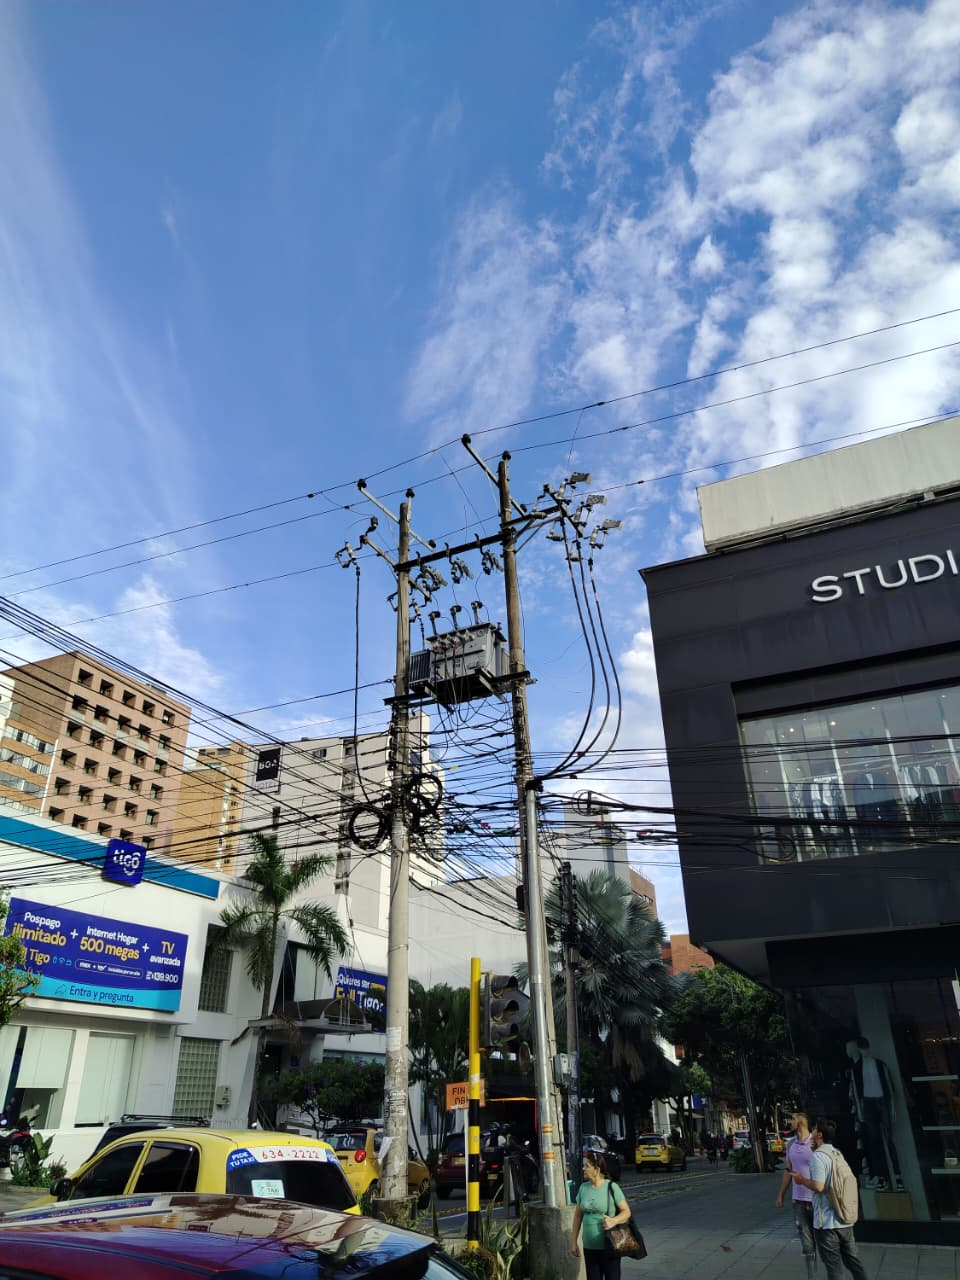
\includegraphics[width=0.43\textwidth, height=0.43\textwidth]{fig_/8}
    \caption{Poste doble de concreto que soporta un transformador de distribución y una compleja red de cableado aéreo de media y baja tensión, así como de telecomunicaciones. La imagen, tomada en una zona comercial concurrida, muestra la densidad de la infraestructura eléctrica en el sector.}
    \label{fig:a8}
\end{figure}

\begin{figure}[H]
    \centering
    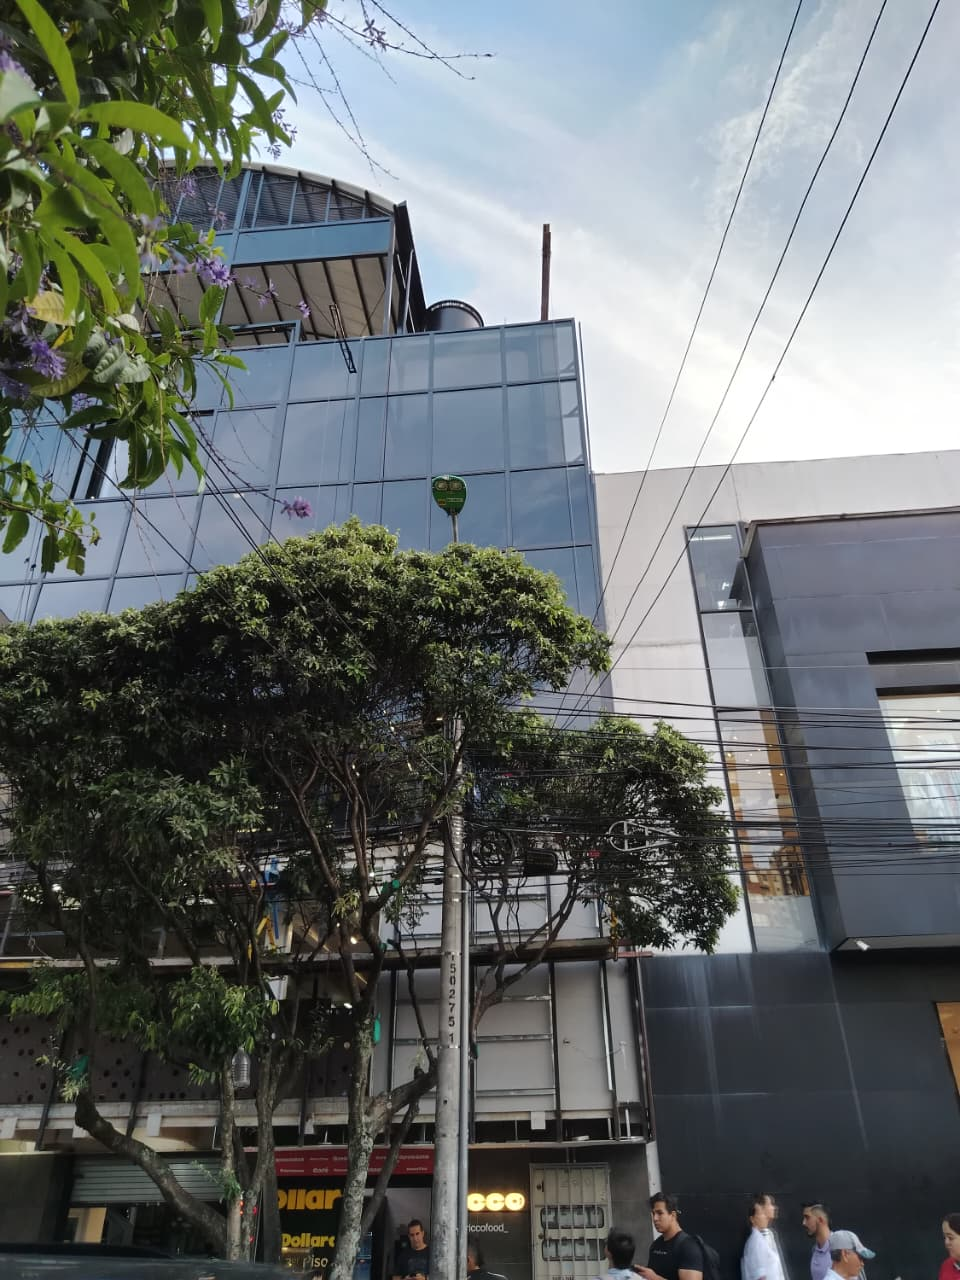
\includegraphics[width=0.43\textwidth, height=0.43\textwidth]{fig_/9}
    \caption{Edificio moderno con fachada de vidrio en una zona comercial. Un árbol frondoso crece junto a un poste de concreto, con sus ramas muy cerca de los cables de la red eléctrica, lo que evidencia un riesgo potencial para la infraestructura y los transeúntes.}
    \label{fig:a9}
\end{figure}

